\chapter{Implementation}


This chapter focuses on the practical implementation of the Domain Legitimacy Checker. The multiviewed approach, along with programming in Python and the web framework in Flask, HTML, CSS, and JavaScript, on the side of external APIs, greatly assisted in making a simple framework for DNS abuse detection and transparency improvement. With these alternatives, a simple but effective method has been developed for determining the legitimacy of domain names, but also for showing clearly the various tactics which bad actors are using in the adoption of confusable domains for phishing and malware distribution, along with other malicious activities to aid with my research. This effort embarked on a journey from idea to execution, focussing on a user-friendly web interface that allows users to quickly identify potentially malicious domains. For further details, refer to the program code listed in the appendix \ref{app:code}.

\section{System Overview}

The development of Domain Legitimacy Checker was chosen because the system is such a robust web-based platform that is tasked with the identification and analysis of domain names that can be malicious. The user first initiates domain name requests through the user interface. This request is processed by the Flask-based web server that orchestrates the core operations of the system. Domain Analysis Engine is meant to perform an analysis on DNS abuse patterns exhibited by the submitted domain using heuristics and pattern matching algorithms. For a detailed check, the system queries external APIs such as VirusTotal for additional legitimacy checks. The results of such checks are kept in a database as well, which gives out the history of known malicious domains. Finally, the Results Display component gives control of the results back to the user. Figure \ref{fig:figfig} provides an illustrative view of the architecture of the software system design and the information flow.


\begin{figure}[H]
\captionsetup{font= footnotesize}
    \centering
    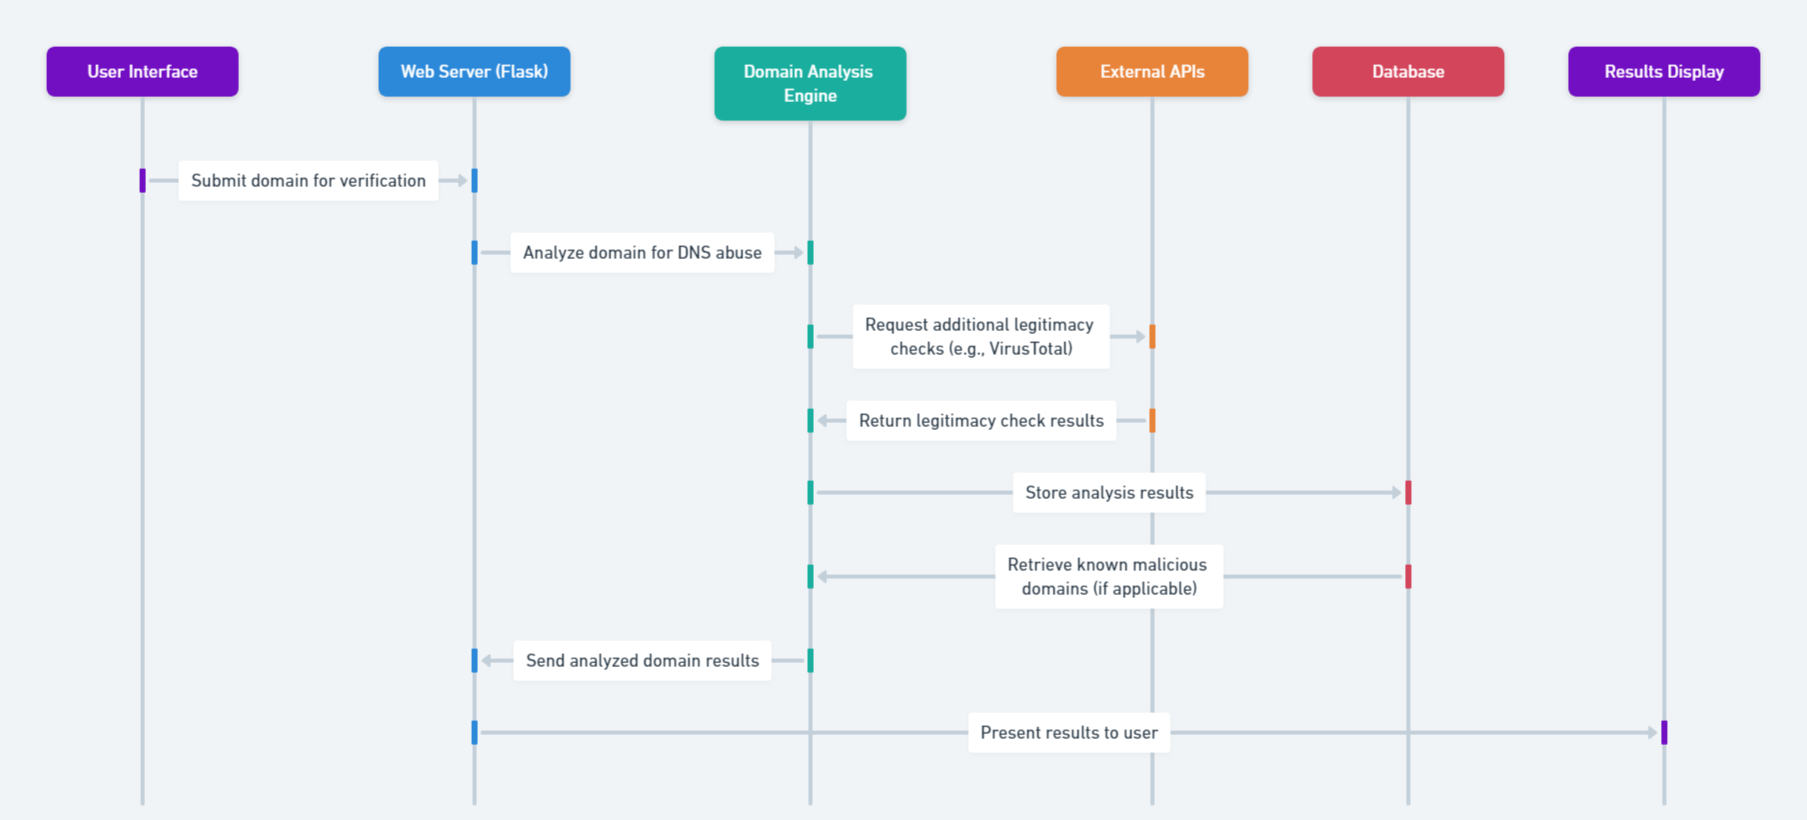
\includegraphics[width=1\linewidth]{project/DNS Abuse Transparency System.png}
    \caption{Domain Legitimacy Checker}
    \label{fig:figfig}
\end{figure}

\section{Tools \& Technologies}

The domain legitimacy checker shown in figure \ref{fig:figfigfig} was built using Python with the use of its third-party modules for development and to provide ways of integration with systems. The platform was powered by Flask, which is a framework that serves requests using the HTTP protocol. The front end is developed using HTML5 in the structuring of web content and is empowered by CSS3 for styling while allowing Bootstrap for a responsive design for all devices. JavaScript provides web pages with simple, interactive, and dynamic functionality. It has also used libraries such as dnspython for the support of DNS queries, which are key in the lookup of domain registration. Request libraries also connect to external APIs such as VirusTotal for the legitimacy analysis of a domain.


It takes advantage of the scanning powers of VirusTotal API, which has several security engines and site scanners to indicate how safe a domain is. It derives its value from domain security, in contrast to the domain name, with thousands of sources and other indicators. Importantly, domains that are already blacklisted to host phishing sites, distribute malware or participate in suspicious activity should be filtered. The choice of each of the tools and technology used was based on its merits but on their integration, making sure that all the systems combined to achieve the cohesiveness and effectiveness of detecting DNS abuse and transparency.



\begin{figure}[H]
    \centering
    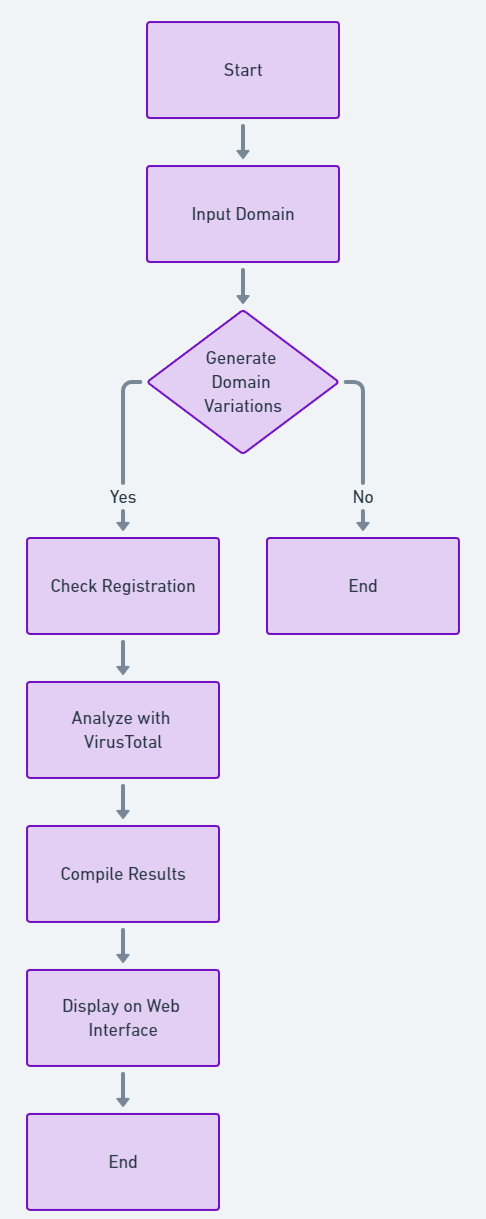
\includegraphics[width=0.6\linewidth]{project/DNS Abuse Inspector Operational Flowchart.png}
    \caption{Domain Legitimacy Checker}
    \label{fig:figfigfig}
\end{figure}
\newpage

\section{Visualisations}

The interface and layout of the web page, as shown in \ref{fig:implem22}, have been designed to facilitate and smooth transition with users. The interface was specially designed so that our users can easily verify whether the domain is legitimate. As with all its applications. Upon loading, the domain legitimacy checker presents itself with a very neat and simple layout. The hero section comes with the name of the application. The domain name input field is at the heart of the page, which requires the user to type the domain url they wish to analyse. Once a domain is submitted, the system jumps into action, processing the input through various checks and analyses. The server logs these interactions, as seen in subsequent visualisations, ensuring that every step of the process is recorded for performance monitoring and optimisation.

\begin{figure}[H]
    \centering
    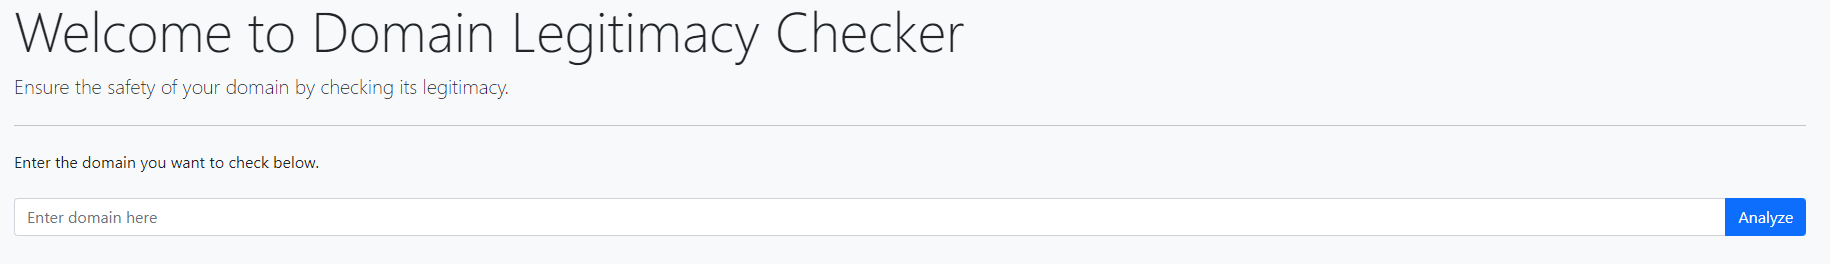
\includegraphics[width=1.1\linewidth]{project/image.png}
    \caption{The main interface of the Domain Legitimacy Checker}
    \label{fig:implem22}
\end{figure}

\subsection{Input \& Interaction}

 The Domain Legitimacy Checker Tool provides a place for interaction with users to ensure a seamless experience, as you can see in \ref{fig:impl2}. The domain input method, a single-field form designed for simplicity of use and quick analysis, is at the centre of this interaction.
 
\begin{figure} [H]
    \centering
    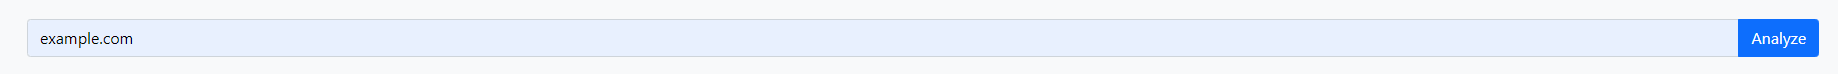
\includegraphics[width=1.1\linewidth]{project/6.png}
    \caption{The domain input box where users begin their interaction with the Domain Legitimacy Checker.}
    \label{fig:impl2}
\end{figure}

First, the user is asked to enter a domain of their choice and to put it in a text box. Right next to the text box is the "Analyze" button as depicted in \ref{fig:imple2222}, contrasting with blue to stand out visually and identify for the user as the next step to take in the process. This design invites immediate action upon domain entry, providing a clear path from user input to results.

\begin{figure}[H]
    \centering
    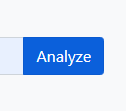
\includegraphics[width=0.1\linewidth]{project/8.png}
    \caption{The 'Analyze' button, poised for user action after domain entry.}
    \label{fig:imple2222}
\end{figure}

The user's request to check a domain is initiated as soon as a domain is entered into the 'Analyze' field and the button is hit: a series of background checks are run to understand the eligibility of the domain. It is at this point with the changing request of the user that his request is no longer an action but a graph analysis that is being done by the systems running in the back end.

\subsection{Interactive Features}

The program comes with an interactive interface; the user is engaged in all the steps from entering a domain for analysis to receiving the results. Starting from the second user having submitted a domain for analysis, this very step will start a circle of HTTP requests, which the server logs with great care. These logs are dynamic, real-time visualisations of user-server interaction rather than just recordings.


The moment a 'click' on the 'Analyze' button happens, the server instantly receives a 'POST' request through the endpoint '/check', which notes that the action marks the start of the domain analysis. On a successful request, a '200' status cookie is returned to signify a successful search. Such types of interaction are logged as entries in the server log, forming a very critical and highly detailed timeline of activities. Figure \ref{fig:imple22222} below visually summarises this process.

\begin{figure}[H]
    \centering
    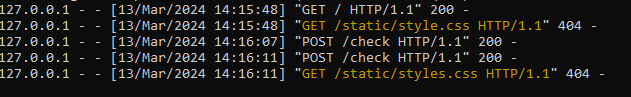
\includegraphics[width=0.8\linewidth]{project/I.png}
    \caption{Server log entries capturing real-time HTTP requests and responses}
    \label{fig:imple22222}
\end{figure}

If there is any issue, these logs are important, for example, in the case of a "404 - Not Found" error in the requested resource. They not only instantly inform system administrators what might have gone wrong, but also act as hints for such troubleshooting. Log analysis allows an administrator to automatically correct problems.

\subsection{Results Display}

The Domain Legitimacy Checker displays the findings in an easy-to-understand style after completion of the domain legitimacy research. Every domain has an icon next to it; an exclamation point indicates that the domain is possibly harmful, and a check mark indicates that the domain is not malicious. The initial level of result interpretation is this visual feedback, which enables users to assess domain safety rapidly."365.com and paypal.com" were tested in figure \ref{fig:1234} and clearly show how the program works when domain names are checked.

\begin{figure}[H]
  \centering
  \begin{subfigure}[b]{0.25\textwidth}
    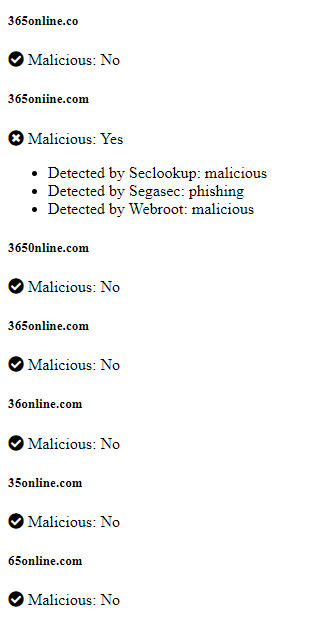
\includegraphics[width=\textwidth]{project/2222.png}
    \label{fig:left}
  \end{subfigure}
  \hfill % adds horizontal space between the figures
  \begin{subfigure}[b]{0.25\textwidth}
    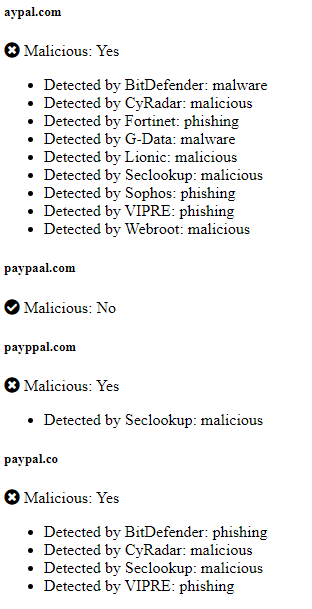
\includegraphics[width=\textwidth]{project/3333.png}
    \label{fig:right}
  \end{subfigure}
  \caption{visual indicators showing the legitimacy status of analysed domains.}
  \label{fig:1234}
\end{figure}

For the malicious domains identified above, the interface unfolds more information as an itemisation of the security threats detected. In each domain, the scanner's findings indicate the exact categories of malicious activities the scanners were able to detect, including malware, phishing, or other security issues. These details are not only comprehensive, but also indicate to the user what might be looked for as the next mitigation step or further investigation. In basic terms, an online brand with such recognition and worldwide users, PayPal is more likely to enter into phishing exploits and use confusable domains compared to the local brand: Bank of Ireland. In this context, although the Bank of Ireland essentially has a local-based client, PayPal does an international scale of operation with huge numbers of clients using their services. Usually, it is a rule that most domain names registered by bad actors closely resemble the official PayPal ones to phish sensitive information from the users. This higher risk factor is directly related to the prominence and wide-reaching scope of PayPal, vis-à-vis a more geographically confined and less known Bank of Ireland.

\subsection{Navigating Results}

After the results from the domain check come back, the Domain Legitimacy Checker would allow the user to easily explore more domains that interest them as shown in figure \ref{fig:sss}. It normally does this through a button that shows on the interface for this function and that simply says "Check Another Domain." This reconnects the user with the input interface.

\begin{figure}[H]
    \centering
    
\includegraphics[width=0.3\linewidth]{project/ii.png}
    \caption{The 'Check Another Domain' button}
    \label{fig:sss}
\end{figure}

This iterative process is another characteristic of the user, so it can be continued non-stop right on the search results page. This squarely builds on the design philosophy of the tool, that of making the user capable of doing as many searches in as lean a manner as possible, fostering an environment of proactive web security.




\section{Challenges \& Solutions}

During the development of the Domain Legitimacy Checker, I faced several challenges, each requiring a tailored solution to ensure the project's success.

Challenge 1: API rate limit
The virus total rate limit API is a very common rate. It is now going to be a problem because it has a limited number of requests and if they exceed that set number, then the service will be temporarily blocked.

Solution: Implement a queuing system with a delay mechanism to spread the requests over time, adhering to the API's rate limits. Additionally, we cached the results of previous queries to minimise repeat requests for the same domains.

Challenge 2: Real-time Feedback for Users, therefore, is important to give instant feedback in the process of the domain analysis, but was otherwise very hard to prove because of the asynchronous behaviour in principle for network operations.in principle for network operations.

Solution: Pass the data to the servers and receive its result from the servers without refreshing the web page using JavaScript. 

Challenge 3: Handling Malicious Domain Variations
Identification and generation of a full set of confusing domain variations represented a key computational challenge.

Solution: Using a combination of common substitution algorithms and a heuristic approach, which prioritised variations based on their likelihood of being used in phishing attacks. 

Challenge 4: Data Storage \& Retrieval Efficiency
Storing analysis results for quick retrieval while managing database performance was a concern, especially with the growth of the data set.

Solution: Implement a real-time domain analysis system with external APIs for comprehensive domain validity checks and the creation of algorithmic domain variations to assess potential security risks. 
 
By addressing these challenges with careful planning and adaptive solutions, we improve the reliability, performance, and user satisfaction of the system.

\section{Testing \& Validation}

The domain legitimacy checker follows rigorous measures in testing the system, which ensures both dependability and accuracy. In the implementation, the back-end logic had a number of things implemented with unit tests; the Python unit test framework was used. The mock objects were used to simulate the acts of external APIs.Manual and automated tests were performed in front-end technologies. Automated UI tests, such as those with Selenium, were used to ensure that all interactive elements are operable. The interface has been tested both automatically and manually, with the help of loading a page on a few browsers and mobile devices to ensure that the interface is responsive and behaves similarly. Continuous Integration (CI) pipelines were set up so that every time a new code commit passes to run tests, ensuring that newly made changes do not break existing functionalities automatically. 

